
\chapter{Inclusion of velocity data} \label{ssn_inclusion_of_velocity_data}

\index{Basal traction}
In order to partition the effects of energy-enhancement and traction-diminishment on momentum -- and thus ensure consistency between rate factor $A(T,W)$ given by (\ref{rate_factor}) and traction coefficient $\beta$ in tangential stress condition (\ref{basal_drag}), (\ref{bp_basal_drag}), (\ref{ps_basal_drag}), and (\ref{rs_basal_drag}) -- an optimization procedure for basal traction is performed for a previously attained energy $\theta$.  Because shear viscosity (\ref{viscosity}), (\ref{bp_viscosity}), (\ref{ps_viscosity}) and (\ref{rs_viscosity}) decreases for increasing energy, the ice speeds up for higher temperature $T$ and water content $W$ due to increased deformation.  Similarly, larger values of basal-traction $\beta$ decrease the vertical average of the mixture velocity while possibly generating more energy due to frictional- and strain-heating.  Indubitably, any generated heat resulting from these processes induces deformation, and therefore also increases the mixture velocity.  Hence a feedback process exists which requires extra care be taken in order to constrain both energy and traction.

An energy constraint already exists as evident by coefficient $W_f$ in rate factor (\ref{rate_factor}); due to lack of empirical evidence, enhancement is limited for ice containing water contents in excess of 1\%.  Regarding basal traction $\beta$, it is desirable to penalize abnormally high spatial gradients in order to reduce non-physical oscillations \citep{vogel_2002}.

The process used to optimize traction coefficient $\beta$ -- referred to in this context as \index{Data assimilation} \emph{data assimilation} -- is directly analogous to the process used to optimize the basal-water content and energy previously described; a momentum objective functional \index{Constrained optimization!Objective function} $\mathscr{I}(\rankone{u}_h, \beta) : \mathcal{H}^1(\Omega) \times \mathcal{H}^1(\Omega) \rightarrow \mathbb{R}$ is minimized over the domain of the ice-sheet $\Omega$.  This objective functional measures the misfit between the observed velocities $\rankone{u}_{ob} = [u_{ob}\ v_{ob}]^\intercal$ and modeled velocities $\rankone{u}_h = [u\ v]^\intercal$ over upper ice-sheet surface $\Gamma_S$,
\begin{align}
  \label{momentum_objective}
  \mathscr{I}(\rankone{u}_h, \beta) = \gamma_1 \mathscr{I}_1(\rankone{u}_h)
                                   + \gamma_2 \mathscr{I}_2(\rankone{u}_h)
                                   + \gamma_3 \mathscr{I}_3(\beta)
                                   + \gamma_4 \mathscr{I}_4(\beta),
\end{align}
where
\begin{align}
  \label{l2_cost}
  \mathscr{I}_1(\rankone{u}_h) = 
    & \frac{1}{2} \int_{\Gamma_S} \left[ (u - u_{ob})^2 + (v - v_{ob})^2 \right] \d{\Gamma_S} \\ 
  \label{logarithmic_cost}
  \mathscr{I}_2(\rankone{u}_h) = 
    & \frac{1}{2} \bigintsss_{\Gamma_S} \ln\left( \frac{ \left(u^2 + v^2\right)^{\nicefrac{1}{2}} + u_0}{\left(u_{ob}^2 + v_{ob}^2\right)^{\nicefrac{1}{2}} + u_0} \right)^2 \d{\Gamma_S} \\ 
  \label{tikhonov_regularization}
  \mathscr{I}_3(\beta) = 
    & \frac{1}{2} \int_{\Gamma_G} \nabla \beta \cdot \nabla \beta \d{\Gamma_G} \\
  \label{tv_regularization}
  \mathscr{I}_4(\beta) = 
    & \int_{\Gamma_G} \left( \nabla \beta \cdot \nabla \beta + \beta_0 \right)^{\nicefrac{1}{2}} \d{\Gamma_G},
\end{align}
with $L^2$ cost coefficient $\gamma_1$, \emph{logarithmic} cost coefficient $\gamma_2$, \index{Constrained optimization!Tikhonov regularization function} \emph{Tikhonov} regularization parameter $\gamma_3$, and \index{Constrained optimization!Total-variation regularization function} \emph{total variation} (TV) regularization parameter $\gamma_4$.  Here, $u_0 = 10\sups{-2}$ and $\beta_0 = 10\sups{-16}$ terms are added to avoid singularities.  Note that the functionals (\ref{l2_cost}) and (\ref{logarithmic_cost}) are referred to as \index{Constrained optimization!Cost function} \emph{cost functionals} while (\ref{tikhonov_regularization}) and (\ref{tv_regularization}) are referred to as \emph{regularization functionals}.

By forming this objective with cost functionals stated in terms of both $L^2$ and logarithmic velocity misfit terms, priority is given to either fast or slow areas of flow by adjusting the values of $\gamma_1$ and $\gamma_2$, respectively \citep{morlighem_2013}.  Note that larger values of $\gamma_3$ and $\gamma_4$ result in increased regularity of $\beta$, at the cost of increased misfit $\left\Vert \rankone{u}_h - \rankone{u}_{ob} \right\Vert$, thus weighting the associated gradient penalty functionals in relation to the other functionals in (\ref{momentum_objective}).  Finally, the addition of the total variation functional (\ref{tv_regularization}) in objective (\ref{momentum_objective}) reduces short-wavelength oscillations that only marginally affect Tikhonov regularization functional (\ref{tikhonov_regularization}).  To my knowledge, this functional has not been used previously for ice-sheet data assimilation.

%===============================================================================
%===============================================================================

\section{Momentum optimization procedure} \label{ssn_momentum_optimization_procedure}

One of the advantages of the action principles presented by \citet{dukowicz_2010} is that action integrals (\ref{action}), (\ref{bp_action}), (\ref{ps_action}), and (\ref{rs_action}) are all self-adjoint.  Indeed, the momentum \index{Constrained optimization!Lagrangian} Lagrangian functional associated with momentum objective (\ref{momentum_objective}) and first-order action principle (\ref{bp_action}) -- used in an analogous set of KKT conditions for momentum as general KKT condition (\ref{barrier_kkt}) -- is defined as
\begin{align}
  \label{momentum_lagrangian}
  \mathscr{H}(\rankone{u}_h, \beta, \rankone{\lambda}) &= \mathscr{I}(\rankone{u}_h, \beta) + \delta_{\rankone{u}_h} \mathcal{A}_{\text{BP}}(\rankone{\lambda}),
\end{align}
with momentum adjoint variable \index{Constrained optimization!Adjoint variable} $\rankone{\lambda} = [\lambda_x\ \lambda_y]^\intercal \in \left( \mathcal{H}^1(\Omega) \right)^2$.

The log-barrier problem \index{Log-barrier method} (see \S \ref{ssn_log_barrier}) for momentum is of the same form as energy barrier problem (\ref{energy_barrier}).  Thus the associated minimization problem for \index{Constrained optimization!Control parameter} control parameter $\beta$ and \index{Constrained optimization!State parameter} state parameter $\rankone{u}_h$ is
\begin{align}
  \min_{\beta}\ \left\{ \varphi_{\omega}(\rankone{u}_h, \beta) = \mathscr{I}(\rankone{u}_h, \beta) - \omega \sum_{i=1}^n \ln(\beta_i) \right\}
\label{momentum_barrier}
\end{align}
for a decreasing sequence of barrier parameters $\omega$ converging to zero, and $n$ is the number of quadrature points in the discretization.  The logarithmic sum term in (\ref{momentum_barrier}) ensures that $\beta$ remains positive, as required by tangential basal stress condition (\ref{basal_drag}).
  
Note that I have used first-order action integral (\ref{bp_action}) in Lagrangian (\ref{momentum_lagrangian}); it has been my experience that solving full-Stokes momentum balance (\ref{extremum}) using a coarse mesh ($\approx$ 1 km minimum cell diameter) and traction $\beta^*$ resulting from the minimization of first-order momentum barrier problem (\ref{momentum_barrier}) results in a velocity field that differs only slightly from that obtained using first-order momentum balance (\ref{bp_extremum}).  This simplification provides a several-fold improvement in computation time.  Note also that the reformulated-Stokes action principle presented in \S \ref{ssn_reformulated_stokes} presents a substantial improvement in the velocity approximation from the first-order model at higher basal gradients (see \S \ref{ssn_ismip_hom_test_simulations}).  However, at its current state of development, \CSLVR has not incorporated this model with the automated adjoint-optimization software it currently employs, Dolfin-Adjoint (\citet{farrell_2013}).
  
Additional computational energy is saved by using a linearization of rate-factor (\ref{rate_factor}) derived from a previously thermo-mechanically coupled $\rankone{u}_h^{i-1}$.  This converts first-order viscosity (\ref{bp_viscosity}) into
\begin{align}
  \label{linear_bp_viscosity}
  \eta_{\text{BP}}^L(\theta, \rankone{u}_h^{i-1}) &= \frac{1}{2}A(\theta)^{-\nicefrac{1}{n}} (\dot{\varepsilon}_{\text{BP}}(\rankone{u}_h^{i-1}) + \dot{\varepsilon}_0)^{\frac{1-n}{n}},
\end{align} 
and first-order-viscous-dissipation term (\ref{bp_viscous_dissipation}) in (\ref{bp_action}) into 
\begin{align}
  \label{linear_viscous_dissipation}
  V^L\left( \dot{\varepsilon}_{\text{BP}}^2 \right) &= 2 \int_0^{\dot{\varepsilon}_{\text{BP}}^2} \eta_{\text{BP}}^L(s) \d{s} 
  = 2 \eta_{\text{BP}}^L\left(\theta, \rankone{u}_h^{i-1} \right) \dot{\varepsilon}_{\text{BP}}^2.
\end{align}
  
Finally, $\delta_{\rankone{u}_h} \mathcal{A}_{\text{BP}}(\rankone{\lambda})$ in Lagrangian (\ref{momentum_lagrangian}) is as derived by \citet{dukowicz_2010},
\begin{align}
  \label{momentum_expanded_lagrangian}
  \mathscr{H}(\rankone{u}_h, \beta, \rankone{\lambda}) =
  &+ \mathscr{I}(\rankone{u}_h, \beta) + \int_{\Gamma_E}\ f_e \rankone{n}_h \cdot \rankone{\lambda} \d{\Gamma_E} \notag \\
  &+ \int_{\Omega} \sigma_{\text{BP}}^L : \nabla \rankone{\lambda} \d{\Omega}
   - \int_{\Omega} \rho g (\nabla S)_h \cdot \rankone{\lambda} \d{\Omega} \notag \\
  &+ \int_{\Gamma_B} \left( \Lambda_{\text{BP}}^L \rankone{\lambda} \cdot \rankone{n}_h + \beta \rankone{u}_h \cdot \rankone{\lambda} \right) \d{\Gamma_B},
\end{align}
where $\sigma_{\text{BP}}^L$ and $\Lambda_{\text{BP}}^L$ are the linearized counterparts to first-order quasi-stress tensor (\ref{bp_stress_tensor}) and impenetrability Lagrange multiplier (\ref{bp_dukowicz_lambda}) utilizing linear viscosity (\ref{linear_bp_viscosity}).

The \CSLVR source code implementation of this procedure is shown in Code Listing \ref{cslvr_u_opt}.

\pythonexternal[label=cslvr_u_opt, caption={\CSLVR source code of the abstract class \texttt{Momentum} for optimizing the velocity and traction.  All of the momentum models of \S \ref{ssn_momentum_and_mass_balance} inherit this method.}, firstline=565, lastline=820]{cslvr_src/momentum.py}

\section{Dual optimization for energy and momentum} \label{ssn_dual_optimization}

To begin the procedure of solving energy and momentum, the thermo-mechanical coupling process described in Algorithm \ref{tmc} is performed for an initial friction field $\beta^i$, energy $\theta^i$, and basal water discharge $F_b^i$.  After this, barrier problem (\ref{momentum_barrier}) is repeatedly solved until the difference between two subsequent traction fields are below a specified tolerance.  This procedure is outlined by Algorithm \ref{tmc_da} with \CSLVR implementation shown in Code Listing \ref{cslvr_tmc_da}.

As suggested by \citet{morlighem_2013}, a suitable initialization of the traction field $\beta^i$ may be formed by vertically integrating first-order momentum balance (\ref{bp_cons_momentum}) and eliminating any horizontal derivatives -- \ie, longitudinal stretching and lateral shearing -- from the left-hand side, resulting in
\begin{align}
  \label{SIA}
  \beta \rankone{u}_h |_B = \rho g H (\nabla S)_h,
\end{align}
where $H = S - B$ is the ice thickness and $\beta \rankone{u}_h |_B$ is the entire contribution of vertical shear, referred to as \emph{basal traction}.  Note that this derivation of the momentum balance is equivalent to the \index{Stokes equations!Applied to ice, shallow ice approximation} \emph{shallow-ice approximation} for glacier flow \citep{greve_2009}.  Finally, using the observed surface velocity as an approximation for basal velocity $\rankone{u}_h |_B$ and taking the norm of vector expression (\ref{SIA}), the shallow-ice-approximate traction field is derived,
\begin{align}
  \label{beta_SIA}
  \beta_{\text{SIA}} = \frac{\rho g H \Vert (\nabla S)_h \Vert}{\Vert \rankone{u}_{ob} \Vert+ u_0},
\end{align}
where $u_0$ is a small positive speed to avoid singularities.  Notice that in areas without surface velocity observations, the approximate traction field (\ref{beta_SIA}) will be invalid.  Therefore, for the purposes of creating an initial traction field, I replace any areas containing missing measurements of velocity $\rankone{u}_{ob}$ in (\ref{beta_SIA}) with the balance velocity $\bar{\rankone{u}}$ as derived in Chapter \ref{ssn_balance_velocity}.

It has been my experience that traction $\beta$ will converge consistently if initialized to the same value prior to solving system (\ref{momentum_barrier}).  Therefore, at the start of every iteration, $\beta$ is reset to its initial value $\beta^i$.  See Algorithm \ref{tmc_da} for details, and Chapter \ref{ssn_application_jakobshavn} for an example of the full energy and momentum optimization procedure applied to the region of Greenland's Jakobshavn Glacier.  In the example that follows, we solve an isothermal momentum-optimization problem.

\begin{algorithm}
  \begin{algorithmic}[1]
    \Function{TMC\_DA}{$\beta^i, \theta^i, F_b^i, n_{\max}$}
      \State $\phantom{\theta,F_b}\mathllap{a_{tol}} := 100$
      \State $\phantom{\theta,F_b}\mathllap{r} := \infty$
      \State $\phantom{\theta,F_b}\mathllap{i} := 1$
      \State $\phantom{\theta,F_b}\mathllap{\beta^p} := \beta^i$
      \State $\theta, F_b := \text{ TMC} \left( \beta^i, \theta^i, F_b^i \right)$
      \While{$r > a_{tol}$ \textbf{and} $i < n_{\max}$}
        \State $\phantom{\theta,F_b}\mathllap{\beta} := \beta^i$
        \State $\phantom{\theta, F_b}\mathllap{\beta^*} := \argminl_{\beta} \Big\{ \varphi_{\omega}(\beta) \Big\}$
        \State $\theta, F_b := \text{TMC} \left( \beta^*, \theta, F_b \right)$
        \State $\phantom{\theta, F_b}\mathllap{r} := \Vert \beta^p - \beta^* \Vert_{2}$
        \State $\phantom{\theta, F_b}\mathllap{\beta^p} := \beta^*$
        \State $\phantom{\theta, F_b}\mathllap{i} := i + 1$
      \EndWhile
      \State \Return $\beta^*$
    \EndFunction
  \end{algorithmic}
  \caption[Thermo-mechanically coupled data-assimilation]{ -- TMC basal-friction data assimilation}
  \label{tmc_da}
\end{algorithm}

\pythonexternal[label=cslvr_tmc_da, caption={Implementation of Algorithm \ref{tmc_da} by \CSLVR contained in the \texttt{Model} class for the optimization of a \texttt{Momentum} and \texttt{Energy} instance.}, firstline=2395, lastline=2586]{cslvr_src/model.py}

%===============================================================================

\section{L-curve analysis} \label{ssn_l_curve}

\index{Constrained optimization!L-curve analysis}
\index{L-curve analysis|seealso{Constrained optimization!L-curve analysis}}
In order to determine the correct values of $\gamma_3$ and $\gamma_4$, we use a process referred to as \emph{L-curve analysis} developed by \citet{hansen_1992}.  The method relies on the fact that for many inverse problems, the shape of the curve resulting from plotting the regularization functional values against the cost functional values for a series of regularization parameters resembles the shape of an `L'.  The `corner' of this curve approximately corresponds to the point whereby increasing regularization begins to negatively impact the cost functional minimization with negligible improvement in smoothness of the control parameter.  One might say that the `cost' of regularization after this point becomes too high.

To this end, we have created the function \texttt{L\_curve} contained within the \texttt{Model} class (Code Listing \ref{cslvr_l_curve}) for automatically performing this calculation for any child class of the \CSLVR \texttt{Physics} class (Code Listing \ref{cslvr_physics}).  All of the physics calculations presented in \S \ref{ssn_momentum_and_mass_balance}, \S \ref{ssn_internal_energy_balance}, \S \ref{ssn_balance_velocity}, \S \ref{ssn_stress_balance}, and \S \ref{ssn_ice_age} inherit from this class; this is because any physics calculation may have an application as an optimization problem.  In regards to momentum objective (\ref{momentum_objective}), we plot the values of the total cost functional $\mathscr{I} = \mathscr{I}_1 + \mathscr{I}_2$ versus either regularization functional $\mathscr{I}_3$ or $\mathscr{I}_4$.

In \S \ref{ssn_ismip_hom_inverse_sims} we examine this procedure for a similar problem as that presented in \S \ref{ssn_ismip_hom_test_simulations}.  Finally, this method was also employed to derive the regularization parameters utilized to generate the simulations presented in Chapter \ref{ssn_application_jakobshavn}.

\pythonexternal[label=cslvr_physics, caption={\CSLVR source code for the abstract class \texttt{Physics} from which all physics calculation classes inherit.}]{cslvr_src/physics.py}

\pythonexternal[label=cslvr_l_curve, caption={\CSLVR implementation of the L-curve procedure of \S \ref{ssn_l_curve}.  Both the cost and regularization functional values are saved as \texttt{txt} files; and plots of the convergence behavior and L-curve as \texttt{pdf} files.}, firstline=2588, lastline=2814]{cslvr_src/model.py}

\section{Ice-shelf inversion procedure} \label{ssn_shelf_inversion}

\index{Flow enhancement factor}
\index{Shelf inversion|seealso{Flow enhancement factor}}
Due to the fact that basal traction $\beta$ defined over floating ice-shelves is very close to zero \citep{greve_2009}, a different control parameter must be specified in order to match the surface velocity observations in these areas.  One choice for this control is enhancement factor $E$ in flow-rate factor (\ref{rate_factor}).  The inversion for this parameter has been used to generate preliminary continent-scale inversions of Antarctica with low error velocity misfit $\Vert \rankone{u} - \rankone{u}_{ob} \Vert$ over ice-shelves.  We only make note of the fact that this option is easily implemented with \CSLVR, and results in a depth-varying distribution of enhancement $E$.

%===============================================================================

\section{ISMIP-HOM inverse test simulation} \label{ssn_ismip_hom_inverse_sims}

\index{Linear differential equations!3D}
\index{ISMIP-HOM simulations}
For a simple test of the momentum optimization procedure described in \S \ref{ssn_momentum_optimization_procedure}, an inverse form of the ISMIP-HOM project presented previously in \S \ref{ssn_ismip_hom_test_simulations} is performed \citep{pattyn_2008}.  This test is defined over the domain $\Omega \in [0,\ell] \times [0,\ell] \times [B,S] \subset \R^3$ with $k_x \times k_y \times k_z$ node discretization, and specifies the use of a surface height with uniform slope $\Vert \nabla S \Vert = a$
\begin{align*}
  S(x) = - x \tan\left( a \right)
\end{align*}
and basal topography matching the surface slope
\begin{align*}
  B(x,y) = S(x) - H,
\end{align*}
with ice thickness $H$.  As before, we enforce continuity via the periodic $\rankone{u}$ boundary conditions (the first-order momentum model does not solve for pressure $p$)
\begin{align*}
  \rankone{u}(0,0)    &= \rankone{u}(\ell,\ell) \\
  \rankone{u}(0,\ell) &= \rankone{u}(\ell,0) \\
  \rankone{u}(x,0)    &= \rankone{u}(x,\ell) \\
  \rankone{u}(0,y)    &= \rankone{u}(\ell,y).
\end{align*}

To begin, first-order momentum system (\ref{bp_extremum}) is solved using the `true' basal traction field
\begin{align*}
  \beta_{\text{true}}(x,y) = \left( \frac{\beta_{max}}{2} \right) \sin\left( \frac{2\pi}{\ell} x \right)\sin\left( \frac{2\pi}{\ell} y \right) + \left( \frac{\beta_{max}}{2} \right)
\end{align*}
with maximum value $\beta_{max}$ (Figure \ref{inverse_ismip_true}).  Similar to \citet{petra_2012}, we add normally-distributed-random noise to the resulting `true' velocity field $\rankone{u}_{\text{true}}$ with standard deviation $\sigma$ to create the simulated `observed' velocity
\begin{align*}
  \rankone{u}_{ob} = \rankone{u}_{\text{true}} + \rankone{\epsilon} 
\end{align*}
where 
\begin{align*}
  \rankone{\epsilon} \distras{iid}\mathcal{N}\left(\rankone{0},\sigma^2 I \right), \hspace{10mm} \sigma = \frac{\Vert \rankone{u}_{\text{true}} \Vert_{\infty}}{\text{SNR}}
\end{align*}
with signal-to-noise ratio SNR (Figure \ref{inverse_ismip_true}).

For simplicity, we use the isothermal rate-factor $A = 10\sups{-16}$  for use with viscosity $\eta$, thus removing the necessity to optimize energy $\theta$.  Table \ref{ismip_hom_inverse_values} lists the coefficients and values used.

To begin the inversion process, $L^2$ cost functional coefficient $\gamma_1$ and logarithmic cost functional coefficient $\gamma_2$ in (\ref{momentum_objective}) are determined by solving momentum optimization problem (\ref{momentum_barrier}) and adjusting their relative values such that at the end of the optimization their associated functionals are of approximately the same order.  Following \citet{morlighem_2013}, we set $\gamma_1 = 1$ and derive by this process $\gamma_2 = 10\sups{5}$ (Figures \ref{ismip_l_curve_convergence_tik} and \ref{ismip_l_curve_convergence_tv}).

The next step is to derive a proper value for the regularization parameters $\gamma_3$ and $\gamma_4$ associated respectively with Tikhonov regularization functional (\ref{tikhonov_regularization}) and total variation regularization functional (\ref{tv_regularization}).  To this end, we perform the L-curve procedure described in \S \ref{ssn_l_curve} over a range of Tikhonov parameters $\gamma_3$ and TV parameters $\gamma_4$ in objective (\ref{momentum_objective}) (see Code Listing \ref{cslvr_l_curve_script}).  For simplicity, we vary only one of $\gamma_3$ or $\gamma_4$ and set the other to zero (Figures \ref{ismip_l_curve_tik} and \ref{ismip_l_curve_tv}).

Results generated with Code Listing \ref{cslvr_inverse_ismip_script} indicate that an appropriate value for both parameters is $\gamma_3, \gamma_4 = 100$.  However, the traction field resulting from Tikhonov regularization with $\gamma_3 = 100$, $\gamma_4=0$ are much more irregular than the results obtained using TV-regularization with $\gamma_3=0$, $\gamma_4=100$ (compare Figures \ref{inverse_ismip_opt_tv} and \ref{inverse_ismip_opt_tikhonov_100}).  Results obtained using Tikhonov-regularization with $\gamma_3=500$, $\gamma_4=0$ produced a qualitatively-smoother result, closer to that obtained via TV-regularization with $\gamma_3=0$, $\gamma_4=100$ (Figure \ref{inverse_ismip_opt_tikhonov_500}).

We conclude by noting that the L-curve procedure described in \S \ref{ssn_l_curve} is a means to derive values for regularization parameters that are \emph{approximately} optimal \citep{vogel_2002}.  Thus simulation and examination of results may be required in order to derive an appropriate value for these parameters.  Additionally, when the true value of the unknown quantity is known, such as the case here, the regularization parameter may be chosen to minimize the error $\Vert \rankone{u}^* - \rankone{u}_{\text{true}} \Vert$.  Real-world data assimilations such as the one presented in Chapter \ref{ssn_application_jakobshavn} do not include `true' values for the velocity, and so we must rely on the technique of trial-and-error to derive these parameters.

\begin{table}
\centering
\caption[Inverse ISMIP-HOM variables]{ISMIP-HOM inverse variables.}
\label{ismip_hom_inverse_values}
\begin{tabular}{llll}
\hline
\textbf{Variable} & \textbf{Value} & \textbf{Units} & \textbf{Description} \\
\hline
$\dot{\varepsilon}_0$ & $10\sups{-15}$ & a\sups{-1}   & strain regularization \\
$A$       & $10\sups{-16}$  & Pa\sups{-3}a\sups{-1}   & flow-rate factor \\
$\ell$    & $20$            & km & width of domain \\
$a$       & $0.5$           & $\circ$                 & surface gradient mag. \\
$H$       & $1000$          & m & ice thickness \\
$\beta_i$ & $\beta_{\text{SIA}}$   & kg m\sups{-2}a\sups{-1} & ini.~traction coef. \\
SNR &     $100$   & -- & $\rankone{u}_{ob}$ signal-to-noise ratio \\
$\gamma_1$ & $10^{-2}$ & kg m\sups{-2}a\sups{-1} & $L^2$ cost coefficient \\
$\gamma_2$ & $5 \times 10^3$ & J a\sups{-1} & log. cost coefficient \\
$\gamma_3$ & $10^{-1}$ & m\sups{6}kg\sups{-1}a\sups{-1} & Tikhonov reg. coef. \\
$\gamma_4$ & $10$ & m\sups{6}kg\sups{-1}a\sups{-1} & TV reg. coeff. \\
$F_b$     & $0$             & m a\sups{-1}            & basal water discharge \\
$k_x$     & $15$            & -- & number of $x$ divisions \\
$k_y$     & $15$            & -- & number of $y$ divisions \\
$k_z$     & $5$             & -- & number of $z$ divisions \\
$N_e$     & $6750$          & -- & number of cells \\
$N_n$     & $1536$          & -- & number of vertices \\
\hline
\end{tabular}
\end{table}

\pythonexternal[label=cslvr_l_curve_script, caption={\CSLVR script for performing the L-curve procedure.}]{scripts/data_assimilation/L_curve.py}

\pythonexternal[label=cslvr_inverse_ismip_script, caption={\CSLVR script used to solve the inverse ISMIP-HOM experiment with regularization parameters derived by Code Listing \ref{cslvr_l_curve_script}.}]{scripts/data_assimilation/ISMIP_HOM_C_inverse.py}


\begin{figure*}
  \centering
    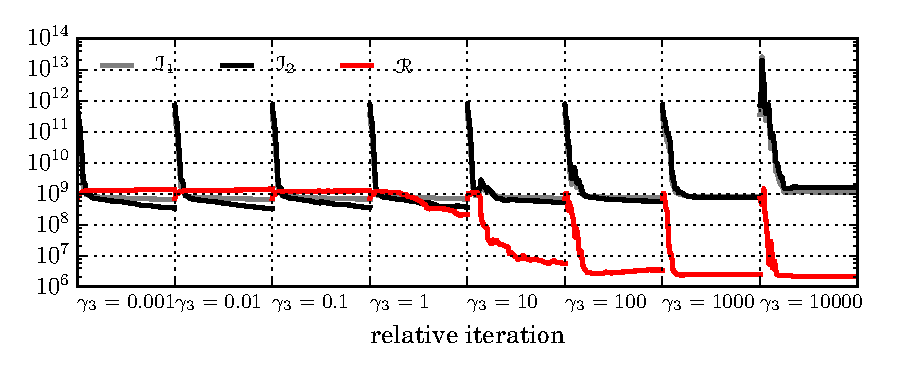
\includegraphics[width=\linewidth]{images/data_assimilation/l_curve/Tikhonov_convergence.pdf}
    \caption[Tikhonov-regularized inverse ISMIP-HOM convergence diagram]{Convergence plot of the cost functional $\gamma_1 \mathscr{I}_1$ (grey) and $\gamma_2 \mathscr{I}_2$ (black), and the Tikhonov regularization functional $\mathscr{I}_3$ (red) for each of the Tikhonov-regularization parameters $\gamma_3$ shown on the $x$-axis.  For this procedure, the TV-regularization parameter $\gamma_4 = 0$, and cost functional coefficient chosen to be $\gamma_1 =1$, $\gamma_2 = 10^5$.}
  \label{ismip_l_curve_convergence_tik}
\end{figure*}

\begin{figure*}
  \centering
    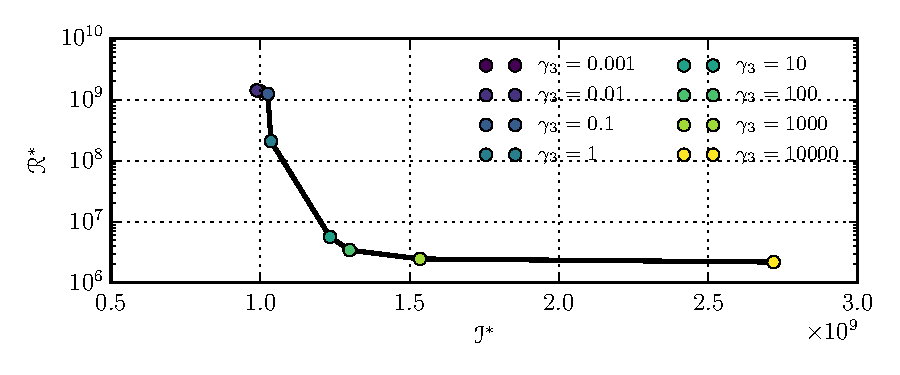
\includegraphics[width=\linewidth]{images/data_assimilation/l_curve/Tikhonov_l_curve.pdf}
    \caption[ISMIP-HOM Tikhonov L-curve diagram]{L-curve for Tikhonov parameter $\gamma_3$ with $\gamma_4=0$.}
  \label{ismip_l_curve_tik}
\end{figure*}

\begin{figure*}
  \centering
    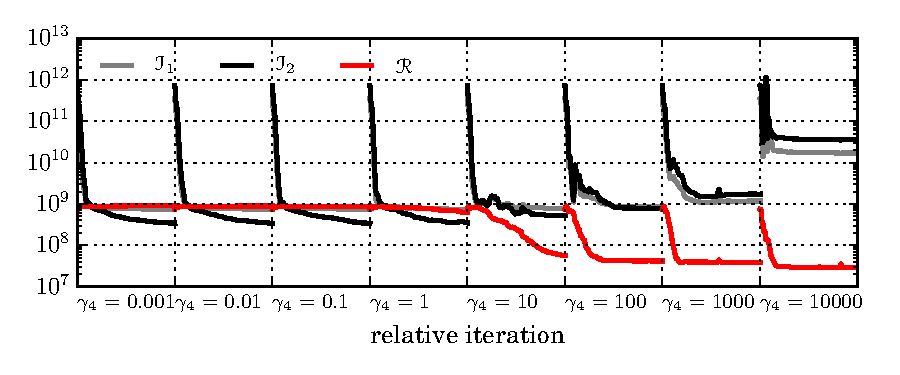
\includegraphics[width=\linewidth]{images/data_assimilation/l_curve/TV_convergence.pdf}
    \caption[Total-variation regularized ISMIP-HOM convergence diagram]{Convergence plot of the cost functional $\gamma_1 \mathscr{I}_1$ (grey) and $\gamma_2 \mathscr{I}_2$ (black), and the TV regularization functional $\mathscr{I}_4$ (red) for each of the TV-regularization parameters $\gamma_4$ shown.  For this procedure, the Tikhonov-regularization parameter $\gamma_3 = 0$, and cost functional coefficient chosen to be $\gamma_1 =1$, $\gamma_2 = 10^5$.}
  \label{ismip_l_curve_convergence_tv}
\end{figure*}

\begin{figure*}
  \centering
    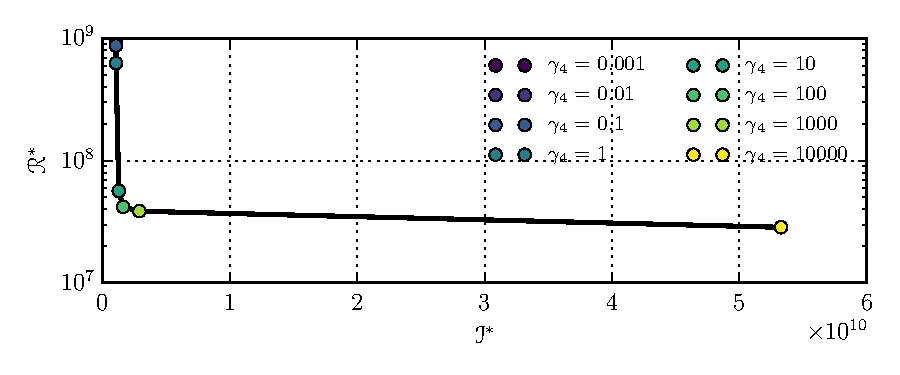
\includegraphics[width=\linewidth]{images/data_assimilation/l_curve/TV_l_curve.pdf}
    \caption[ISMIP-HOM total-variation L-curve diagram]{L-curve for total-variation parameter $\gamma_4$ with $\gamma_3=0$.}
  \label{ismip_l_curve_tv}
\end{figure*}

\begin{figure}
  \centering
    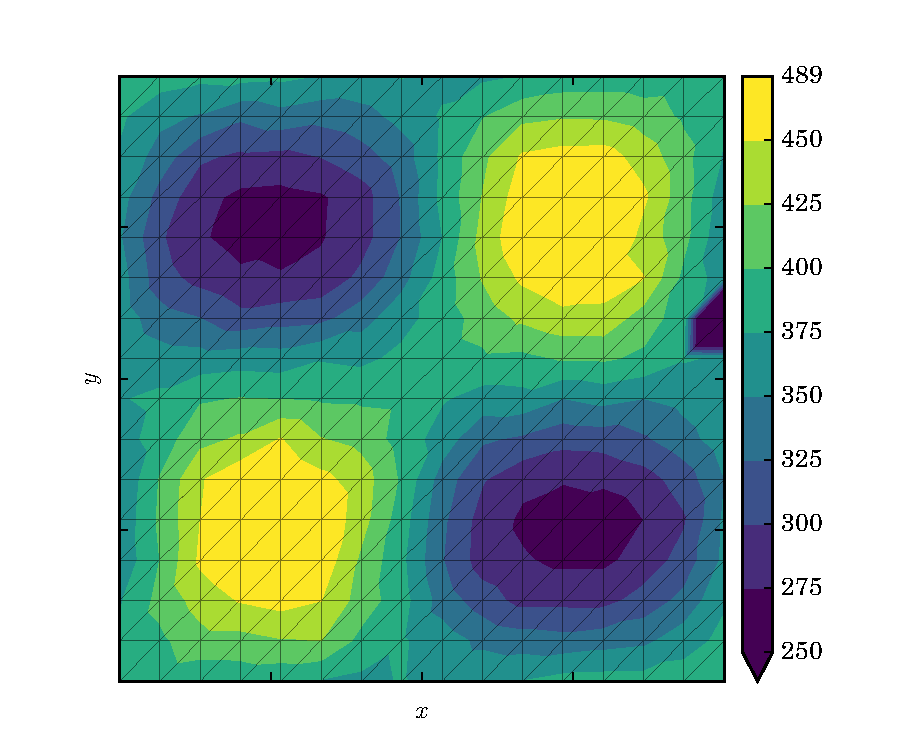
\includegraphics[width=0.9\linewidth]{images/data_assimilation/ISMIP_HOM_C/TV/beta_SIA.pdf}
    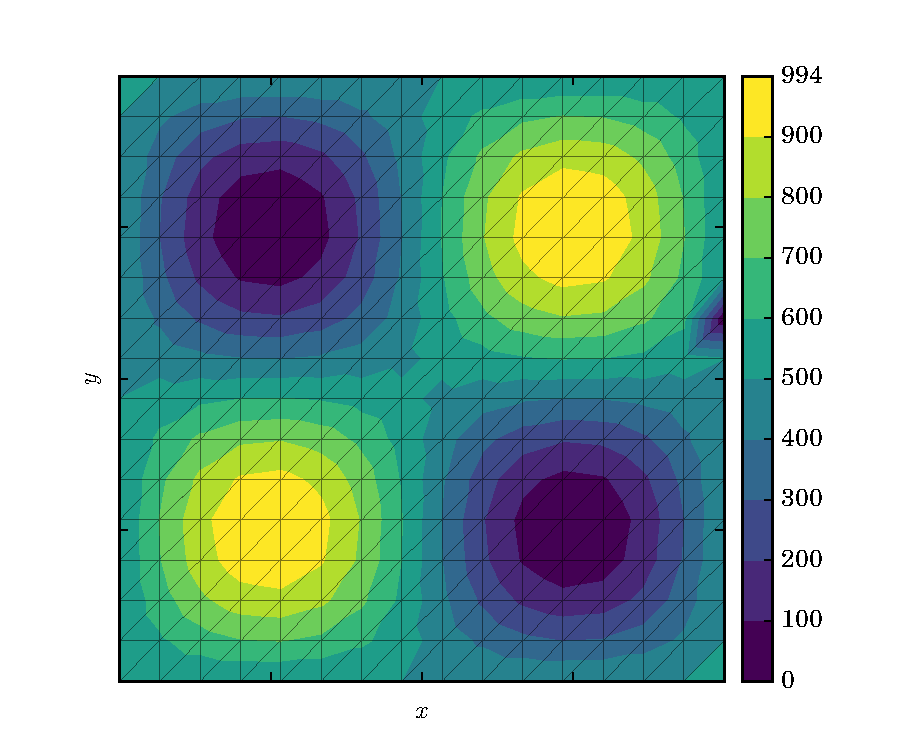
\includegraphics[width=0.9\linewidth]{images/data_assimilation/ISMIP_HOM_C/TV/beta_true.pdf}
    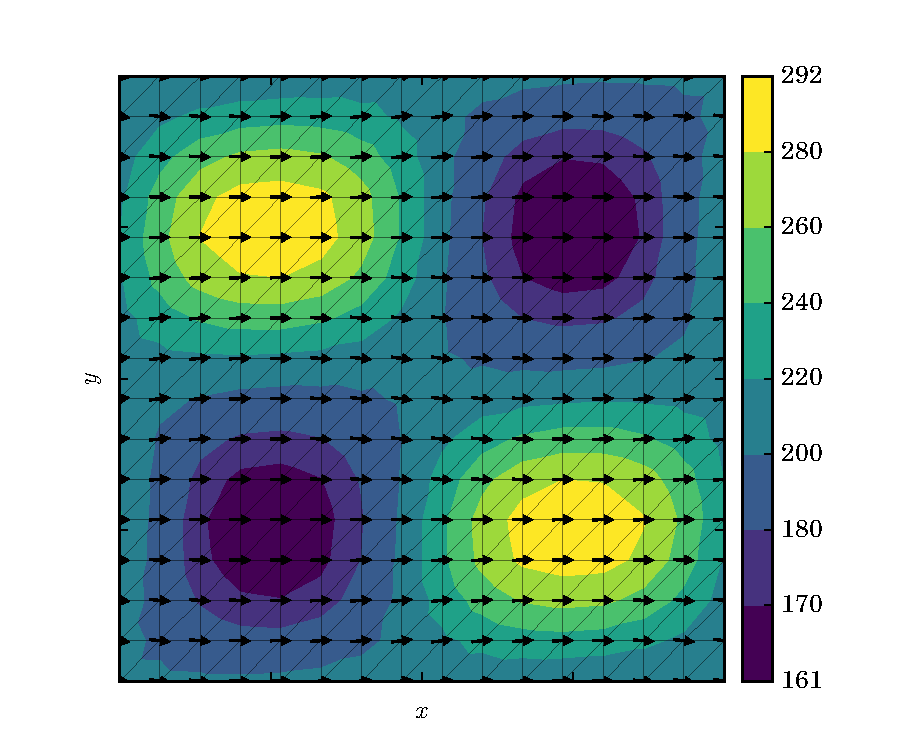
\includegraphics[width=0.9\linewidth]{images/data_assimilation/ISMIP_HOM_C/TV/U_true.pdf}
  \caption[Inverse ISMIP-HOM `true' data fields]{ISMIP-HOM C initial value for traction $\beta$, SIA traction coefficient $\beta_{\text{SIA}}$ (top), `true' traction coefficient $\beta_{\text{true}}$ (middle), and `true' velocity $\rankone{u}_{\text{true}}$ (bottom) with a $20 \times 20$ square km grid.}
  \label{inverse_ismip_true}
\end{figure}

\begin{figure}
  \centering
    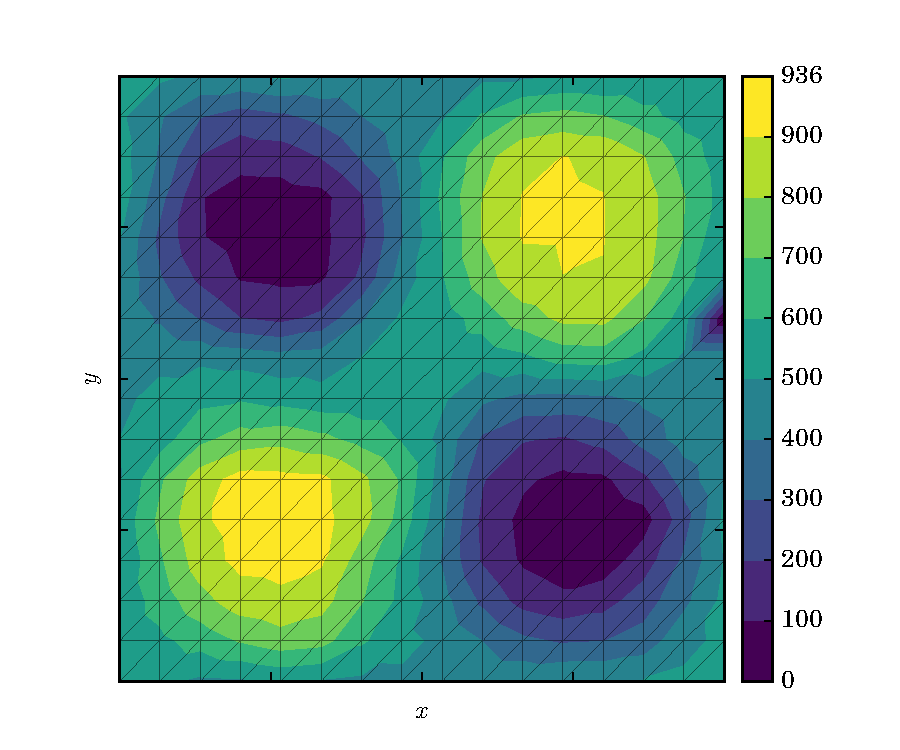
\includegraphics[width=0.9\linewidth]{images/data_assimilation/ISMIP_HOM_C/TV/beta_opt.pdf}
    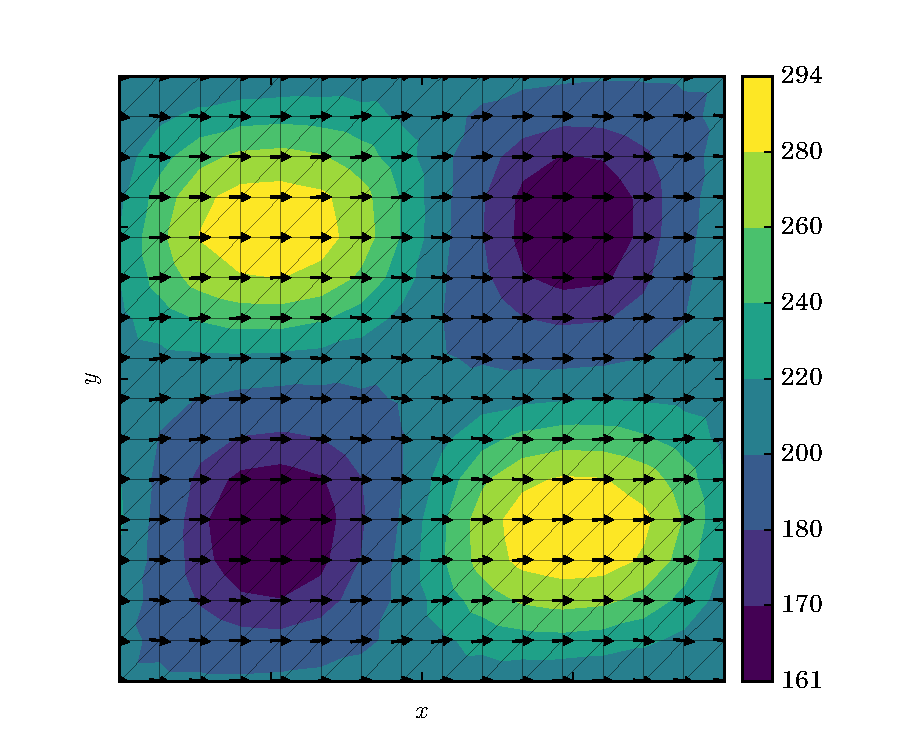
\includegraphics[width=0.9\linewidth]{images/data_assimilation/ISMIP_HOM_C/TV/U_opt.pdf}
    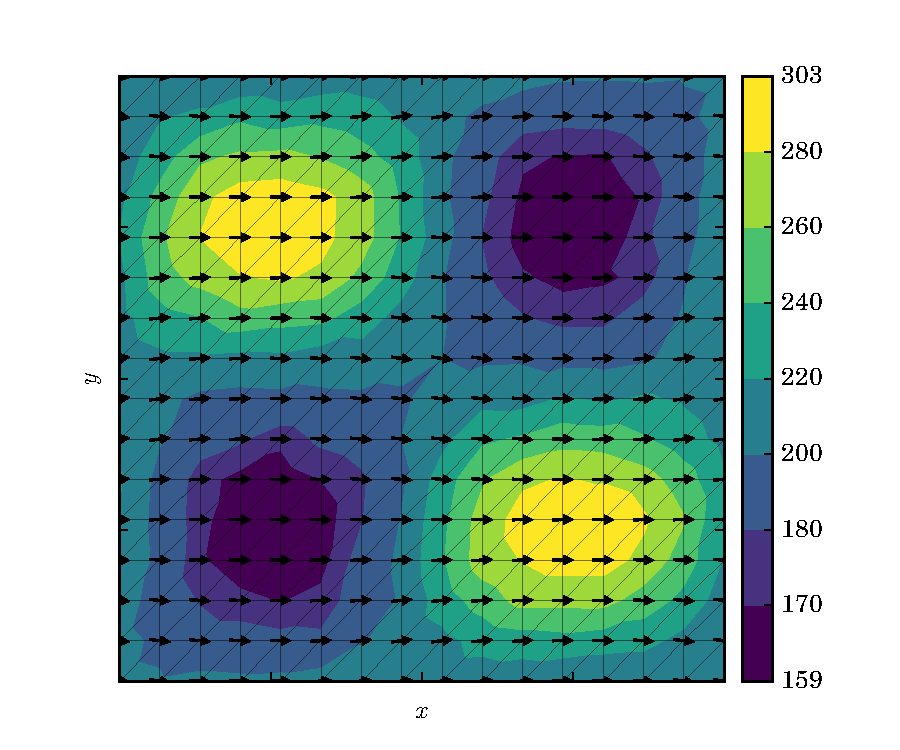
\includegraphics[width=0.9\linewidth]{images/data_assimilation/ISMIP_HOM_C/TV/U_ob.pdf}
  \caption[TV-regularized inverse ISMIP-HOM results]{Results obtained using TV-regularization with $\gamma_3=0$, $\gamma_4=100$; optimized traction coefficient $\beta^*$ (top), optimized velocity $\rankone{u}^*$ (middle), and `observed' velocity $\rankone{u}_{ob}$ (bottom) with a $20 \times 20$ square km grid.}
  \label{inverse_ismip_opt_tv}
\end{figure}

\begin{figure}
  \centering
    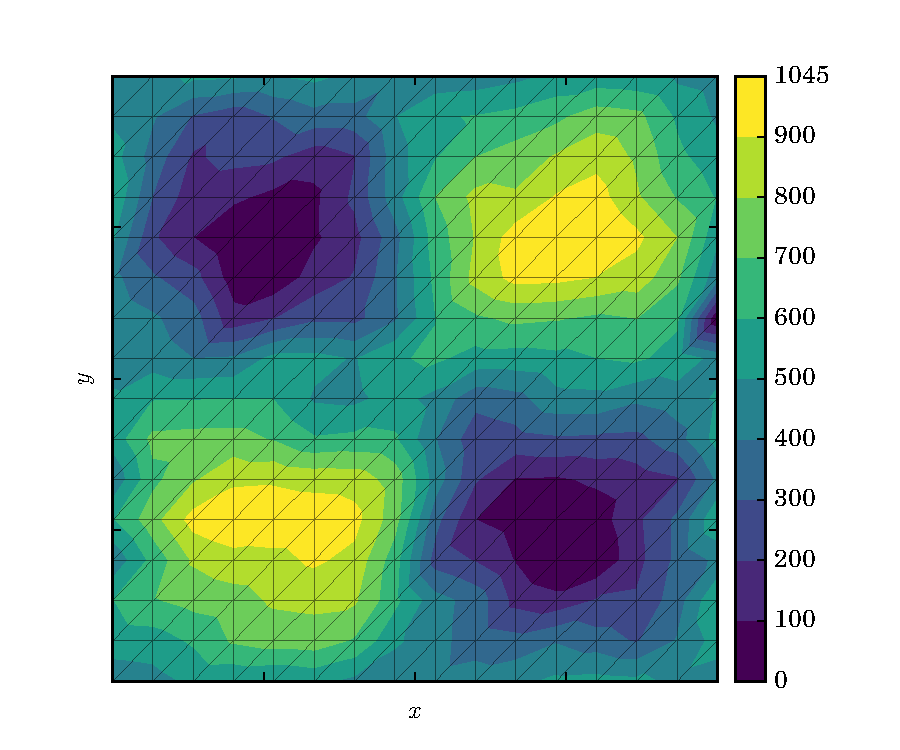
\includegraphics[width=0.9\linewidth]{images/data_assimilation/ISMIP_HOM_C/Tikhonov_100/beta_opt.pdf}
    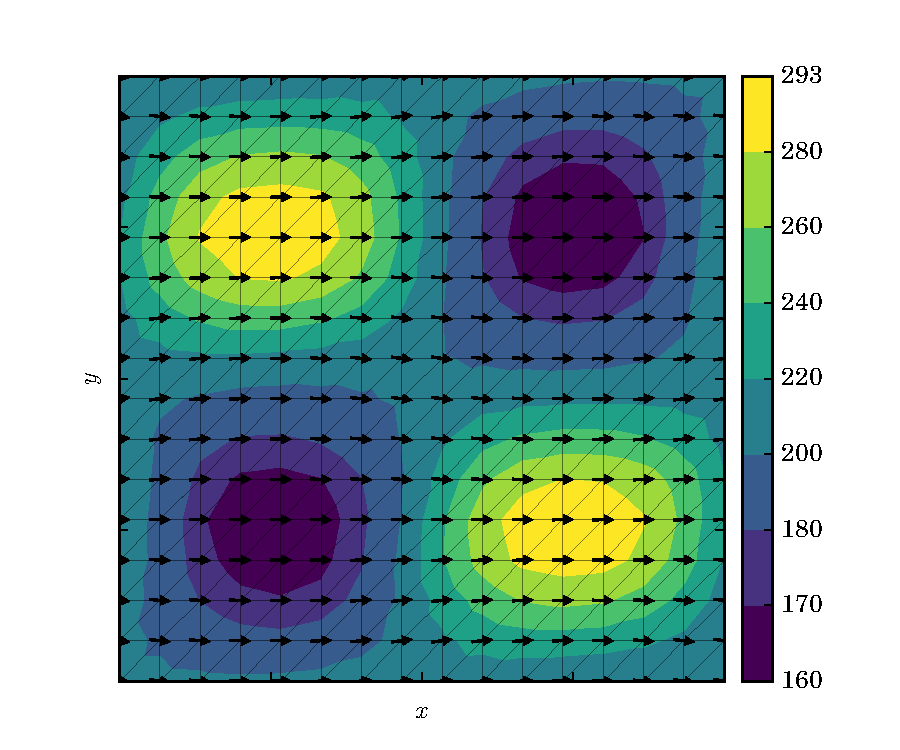
\includegraphics[width=0.9\linewidth]{images/data_assimilation/ISMIP_HOM_C/Tikhonov_100/U_opt.pdf}
    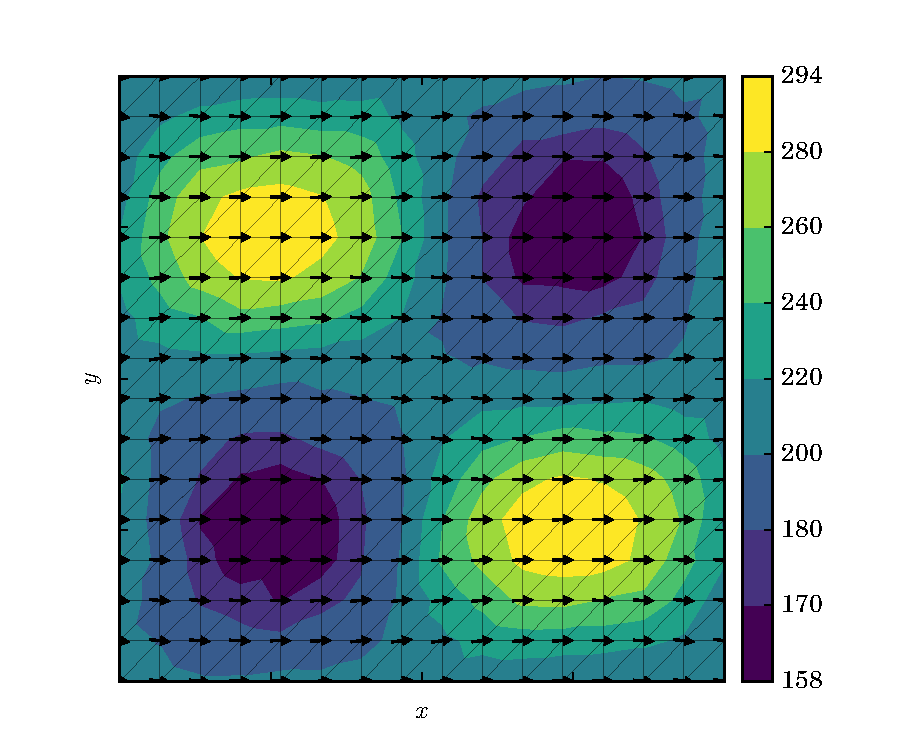
\includegraphics[width=0.9\linewidth]{images/data_assimilation/ISMIP_HOM_C/Tikhonov_100/U_ob.pdf}
  \caption[Tikhonov-regularized inverse ISMIP-HOM results with $\gamma_3=100$]{Results obtained using Tikhonov-regularization with $\gamma_3=100$, $\gamma_4=0$; optimized traction coefficient $\beta^*$ (top), optimized velocity $\rankone{u}^*$ (middle), and `observed' velocity $\rankone{u}_{ob}$ (bottom) with a $20 \times 20$ square km grid.}
  \label{inverse_ismip_opt_tikhonov_100}
\end{figure}

\begin{figure}
  \centering
    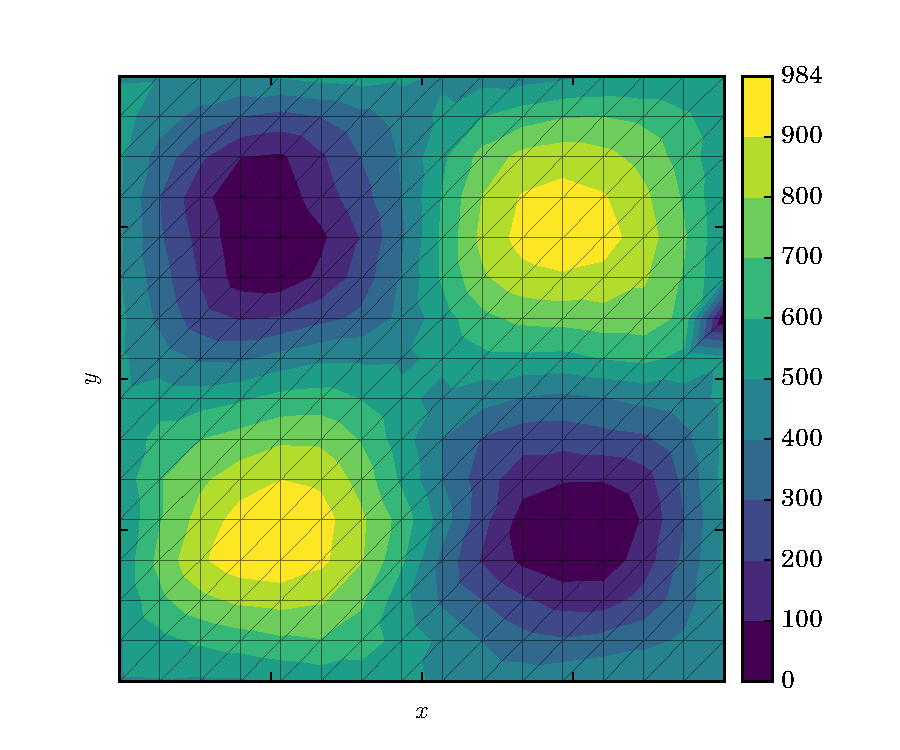
\includegraphics[width=0.9\linewidth]{images/data_assimilation/ISMIP_HOM_C/Tikhonov_500/beta_opt.pdf}
    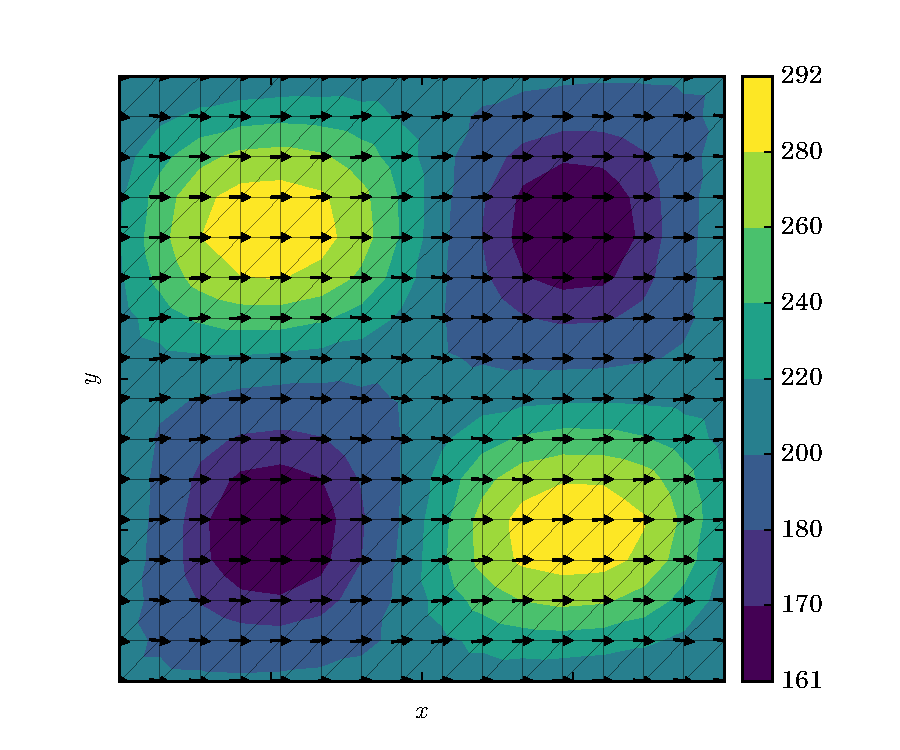
\includegraphics[width=0.9\linewidth]{images/data_assimilation/ISMIP_HOM_C/Tikhonov_500/U_opt.pdf}
    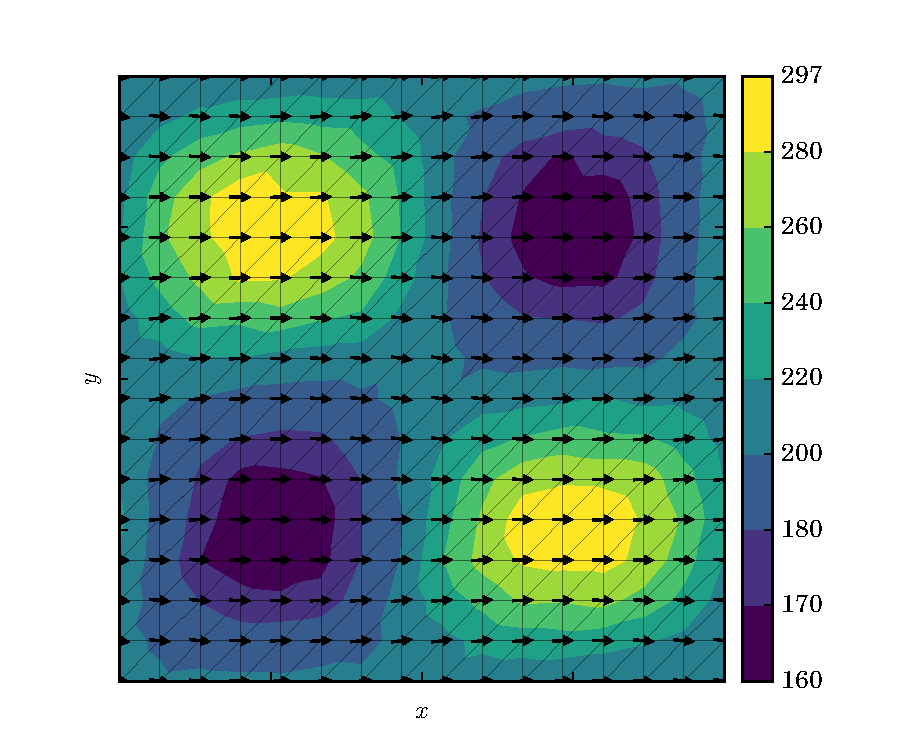
\includegraphics[width=0.9\linewidth]{images/data_assimilation/ISMIP_HOM_C/Tikhonov_500/U_ob.pdf}
  \caption[Tikhonov-regularized inverse ISMIP-HOM results with $\gamma_3=500$]{Results obtained using Tikhonov-regularization with $\gamma_3=500$, $\gamma_4=0$; optimized traction coefficient $\beta^*$ (top), optimized velocity $\rankone{u}^*$ (middle), and `observed' velocity $\rankone{u}_{ob}$ (bottom) with a $20 \times 20$ square km grid.}
  \label{inverse_ismip_opt_tikhonov_500}
\end{figure}
